\chapter{Evaluation Content}
\section{Worksheet}
\subsection{Introduction to Turing Machine Language}
In this section, you are given some programs in Turing Machine Language (TML). They will be used to explain the syntax of the programming language and how they can be run on tapes.
\begin{itemize}
    \item \texttt{isDiv2}:
    \lstinputlisting[language=TML]{code/isDiv2.txt}
    
    \item \texttt{isDiv2Rec}:
    \lstinputlisting[language=TML]{code/isDiv2Rec.txt}

    \noindent Both \texttt{isDiv2} and \texttt{isDiv2Rec} correspond to the following Turing Machine (TM):
    \begin{figure}[H]
        \centering
        \begin{tikzpicture}
            \node[state, accepting] (q0) at (0, 0) {$q_0$};
            \node[state] (q1) at (3, 0) {$q_1$};
            \node[state, fill=green, opacity=0.6] (A) at (6, -1) {$A$};
            \node[state, fill=red, opacity=0.6] (R) at (6, 1) {$R$};

            \draw[->] (q0) edge[loop above] node {$0|1, R$} (q0);
            \draw[->] (q0) -- node[above] {$\#, L$} (q1);
            \draw[->] (q1) -- node[below left] {$0, L$} (A);
            \draw[->] (q1) -- node[above left] {$1|\#, L$} (R);
        \end{tikzpicture}
    \end{figure}
    
    \item \texttt{aNbN}:
    \lstinputlisting[language=TML]{code/aNbN.txt}

    \noindent The program \texttt{aNbN} corresponds to the following TM:
    \begin{figure}[H]
        \centering
        \begin{tikzpicture}
            \node[state, accepting] (q0) at (0, 0) {$q_0$};
            \node[state] (q1) at (0, -2) {$q_1$};
            \node[state] (q2) at (6, -2) {$q_2$};
            \node[state] (q3) at (6, 0) {$q_3$};
            \node[state, fill=green, opacity=0.6] (A) at (-3, 0) {$A$};
            \node[state, fill=red, opacity=0.6] (R) at (3, -1) {$R$};

            \draw[->] (q0) -- node[left] {$a \to \#, R$} (q1);
            \draw[->] (q0) -- node[above] {$\#, L$} (A);
            \draw[->] (q0) -- node[below] {$b, L$} (R);
            \draw[->] (q1) edge[loop below] node {$a|b, R$} (q1);
            \draw[->] (q1) -- node[below] {$\#, L$} (q2);
            \draw[->] (q2) -- node[right] {$b \to \#, L$} (q3);
            \draw[->] (q3) edge[loop above] node {$a|b, L$} (q3);
            \draw[->] (q2) -- node[above] {$a|\#, L$} (R);
            \draw[->] (q3) -- node[above] {$\#, L$} (q0);
        \end{tikzpicture}
    \end{figure}
\end{itemize}

\subsection{Identifying TML Programs}
In this section, you are presented with TML programs. You will be given some tape values to run the program in and decode what values the program accepts. You are encouraged to use the website to try and solve this.

\begin{enumerate}
    \item Consider the following TML Program:
    \lstinputlisting[language=TML]{code/mystery1.txt}

    \begin{enumerate}
        \item Does the program accept the values:
        \begin{enumerate}
            \item $10$ (NOTE: This is $2$ in decimal)
            \item $1$
            \item $100$ (NOTE: This is $4$ in decimal)
            \item $101$ (NOTE: This is $5$ in decimal)
            \item $110$ (NOTE: This is $6$ in decimal)
        \end{enumerate}
        \item Describe the values this program accepts.
    \end{enumerate}
    \newpage

    \item Consider the following TML program:
    \lstinputlisting[language=TML]{code/mystery2.txt}
    \begin{enumerate}
        \item Does the program accept the values:
        \begin{enumerate}
            \item $ab$
            \item $aabb$
            \item $abba$
            \item $bab$
        \end{enumerate}
        
        \item Describe the values this program accepts.
    \end{enumerate}
\end{enumerate}

\newpage

\subsection{Identifying TMs}
In this section, you are presented with TMs. You will be given some tape values to run the program in and decode what values the program accepts. Since the website can only execute TML programs, you are also given the TML program for the code, but it is not comprehensible like the previous programs; you will likely find it easier to understand the TM than the program (which you should do!). 
\begin{enumerate}
    \item Consider the following TM FSM:
    \begin{figure}[H]
        \centering
        \begin{tikzpicture}
            \node[state, accepting] (q0) at (0, 0) {$q_0$};
            \node[state] (q1) at (3, 0) {$q_1$};
            \node[state] (q2) at (6, 0) {$q_2$};
            \node[state, fill=green, opacity=0.6] (A) at (0, -2) {$A$};
            \node[state, fill=red, opacity=0.6] (R) at (4.5, -2) {$R$};

            \draw[->] (q0) edge[loop above] node {$0, R$} (q0);
            \draw[->] (q0) edge[bend right] node[above] {$1, R$} (q1);
            \draw[->] (q1) edge[bend right] node[above] {$1, R$} (q0);
            \draw[->] (q1) edge[bend right] node[above] {$0, R$} (q2);
            \draw[->] (q2) edge[bend right] node[above] {$0, R$} (q1);
            \draw[->] (q2) edge[loop above] node {$1, R$} (q2);
            \draw[->] (q0) edge node[left] {$\#, R$} (A);
            \draw[->] (q1) edge node[left] {$\#, R$} (R);
            \draw[->] (q2) edge node[right] {$\#, R$} (R);
        \end{tikzpicture}
    \end{figure}
    You are given a basic representation of this FSM as code in Teams. The file is called mystery3.
    \begin{enumerate}
        \item Does the TM accept the values:
        \begin{enumerate}
            \item $11$ (NOTE: This is $3$ in decimal)
            \item $10$ (NOTE: This is $2$ in decimal)
            \item $1$
            \item $110$ (NOTE: This is $6$ in decimal)
            \item $1001$ (NOTE: This is $9$ in decimal)
        \end{enumerate}
        
        \item Describe the values this program accepts.
    \end{enumerate} 
    
    \item Consider the following TM FSM:
    \begin{figure}[H]
        \centering
        \begin{tikzpicture}
            \node[state, accepting] (q0) at (3, 0) {$q_0$};
            \node[state] (q1) at (2, -2) {$q_1$};
            \node[state] (q2) at (5, -3) {$q_2$};
            \node[state] (q3) at (8, -2) {$q_3$};
            \node[state] (q7) at (6, 0) {$q_4$};
            \node[state, fill=green, opacity=0.6] (A) at (0, 0) {$A$};
            \node[state, fill=red, opacity=0.6] (R) at (5, -1) {$R$};

            \draw[->] (q0) -- node[left] {$a \to \#, R$} (q1);
            \draw[->] (q0) -- node[above] {$\#, R$} (A);
            \draw[->] (q1) edge[loop below] node {$a|b, R$} (q1);
            \draw[->] (q1) -- node[below left] {$\#, L$} (q2);
            \draw[->] (q2) -- node[below right] {$b \to \#, L$} (q3);
            \draw[->] (q3) -- node[right] {$b \to \#, L$} (q7);
            \draw[->] (q7) edge[loop right] node {$a|b, L$} (q7);
            \draw[->] (q7) -- node[above] {$\#, R$} (q0);
            \draw[->] (q2) -- node[left] {$a|\#, R$} (R);
            \draw[->] (q3) -- node[above] {$a|\#, R$} (R);
            \draw[->] (q0) -- node[below] {$b, R$} (R);
        \end{tikzpicture}
    \end{figure}
    You are given a basic representation of this FSM as code in Teams. The file is called mystery4.
    \begin{enumerate}
        \item Does this TM accept the values:
        \begin{enumerate}
            \item $ab$
            \item $abb$
            \item $aabbbb$            
            \item $bab$
            \item $abba$
        \end{enumerate}

        \item Describe the values this program accepts.
    \end{enumerate}
\end{enumerate}
\newpage


\subsection{Writing TML Programs}

Following a similar syntax to the code given above, write the following programs. You are free to use the website to check the accuracy of the program while writing the programs. Please answer these questions in the survey.
\begin{enumerate}
    \item divisibility by 4 in binary iteratively [HINT: Go to the end and check for 2 zeros. Allow 0 as well.]
    \item divisibility by 4 in binary, recursively.
\end{enumerate}
    
The remaining questions are optional. 
\begin{enumerate}
    \setcounter{enumi}{2}
    \item strings of the form $a^n b^m c^{n+m}$
    \item strings of the form $a^n b^n c^n$
    \item HARD: check there are same number of $a$'s and $b$'s
\end{enumerate}

\section{Checklist}
\section{Survey}
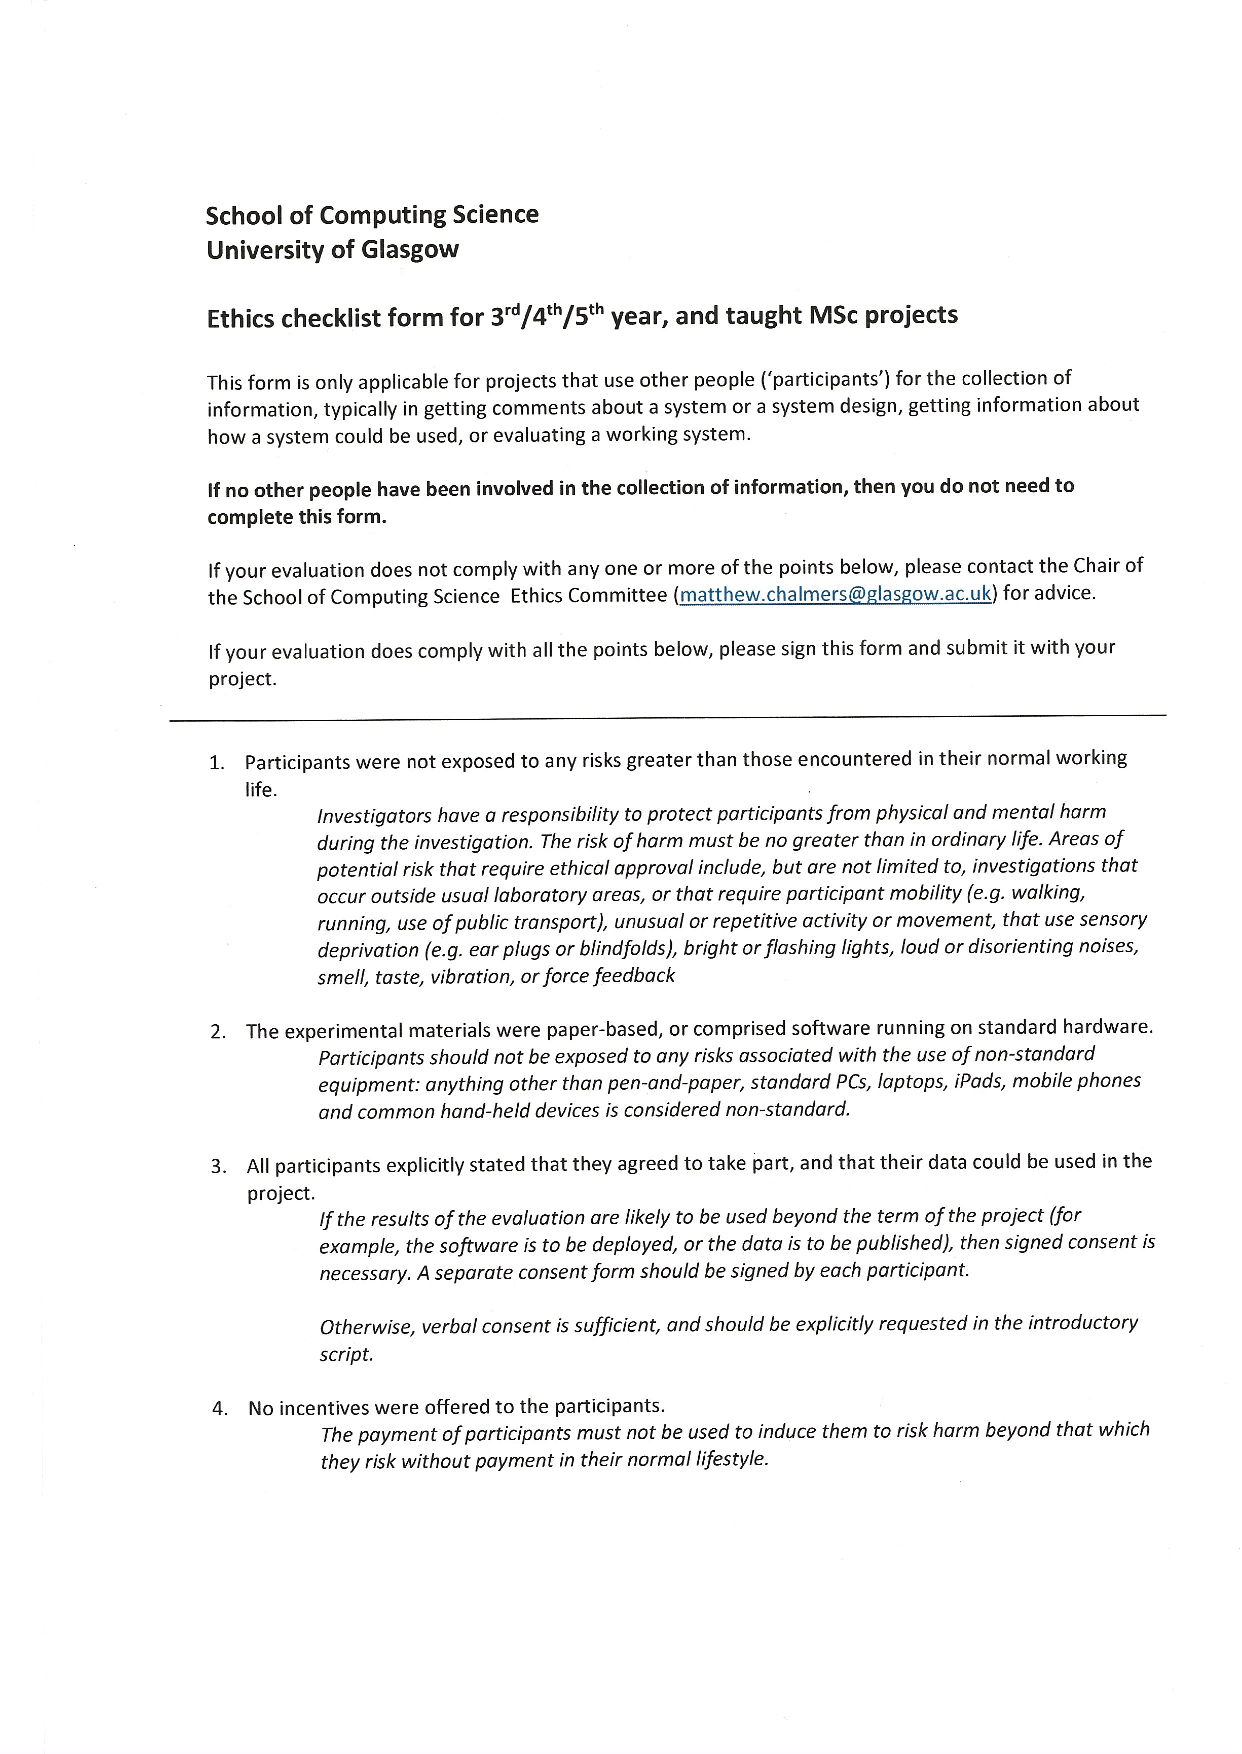
\includepdf[pages=-]{checklist.pdf}
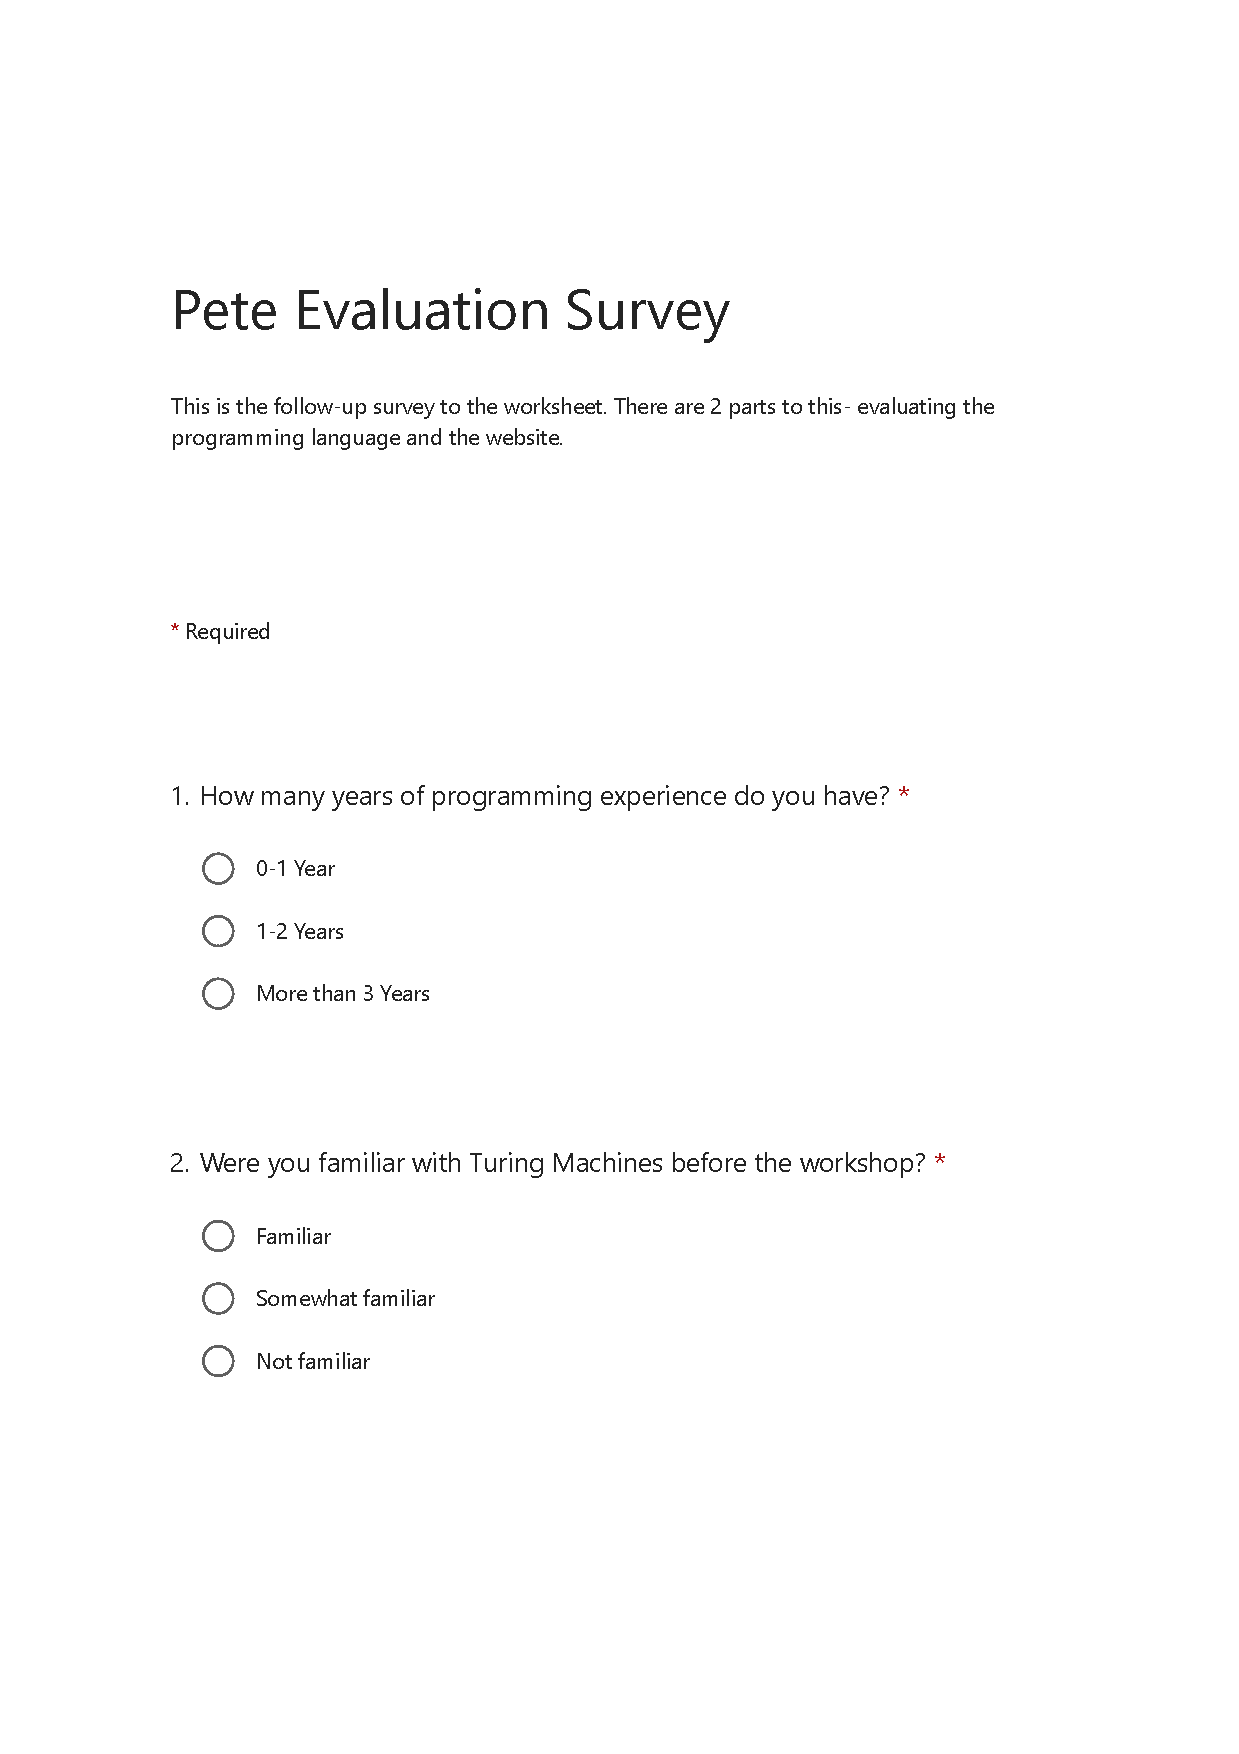
\includepdf[pages=-]{survey.pdf}